%=====================================================================
\section{Resultados en la prueba de 2026}

La configuración congelada se evaluó una sola vez sobre los \cifNPrueba{} commits de enero a julio de 2026 (prevalencia \cifPrevPrueba{}), tras verificar la huella de la partición. La Tabla~\ref{tab:prueba} reúne desempeño y costo.

\begin{table*}[!t]
\caption{Prueba de 2026: desempeño (media de las semillas; IC 95\,\% por \emph{bootstrap} de la semilla de referencia) y costo. Métricas con umbral: el que maximiza el MCC en 2025}
\label{tab:prueba}
\centering\footnotesize
\begin{tabular}{@{}l c c c c c c r r r@{}}
\toprule
\cabecera \textbf{Modelo} & \textbf{AUC-PR} & \textbf{IC 95\,\%} & \textbf{AUC-ROC} & \textbf{MCC} & \textbf{Sensib.} & \textbf{Especif.} & \textbf{Parám.} & \textbf{Entren.\ (s)} & \textbf{ms/1000}\\
\midrule
\filas{../comun/tabla_prueba.tex}
\bottomrule
\end{tabular}
\end{table*}

\subsection{Criterio de éxito}

El proyecto \textbf{no alcanza} el criterio fijado en la Entrega 1:
\begin{itemize}
\item \textbf{C1, desempeño: se cumple.} El difuso-evolutivo logra \cifTestFE{} $\pm$ \cifTestFEde{} de AUC-PR, el \cifCuno{} del \emph{gradient boosting} (\cifTestGB{}). La meta era 90\,\%.
\item \textbf{C2, robustez: no se cumple.} Pierde el \cifCaidaFE{} de su AUC-PR de validación; el \emph{gradient boosting} pierde el \cifCaidaGB{} y la regresión logística el \cifCaidaLR{}.
\item \textbf{C3, piso: se cumple solo en su primera parte.} El IC 95\,\% del AUC-PR, \cifTestFEic{}, excluye la prevalencia, y el modelo multiplica el AUC-PR del azar por cerca de 3,5. Las pruebas de McNemar son significativas ($p<10^{-6}$) contra todas las referencias, pero a favor de ellas, salvo contra la variante sin evolución:
  \begin{itemize}
  \item frente al \emph{gradient boosting}, el difuso acierta donde aquel falla en \cifMcAciertaGB{} commits y falla donde aquel acierta en \cifMcFallaGB{};
  \item frente a la variante sin evolución, las cifras se invierten: \cifMcAciertaVar{} frente a \cifMcFallaVar{}.
  \end{itemize}
\end{itemize}

\textbf{Friedman--Nemenyi.} La prueba de Friedman sobre los cuatro bloques (tres ventanas y la prueba) rechaza la igualdad de los cinco modelos ($p=\cifFriedmanP{}$). Los rangos medios son:
\begin{itemize}
\item \emph{gradient boosting}: \cifRangoGB{};
\item difuso-evolutivo y regresión logística: \cifRangoFE{};
\item variante sin evolución: \cifRangoVar{};
\item clase mayoritaria: \cifRangoMay{}.
\end{itemize}
Con la diferencia crítica de Nemenyi (\cifNemenyiCD{}), solo la distancia entre el \emph{gradient boosting} y la clase mayoritaria es significativa. Con cuatro bloques, la prueba tiene poca potencia.

\subsection{El umbral no se transfiere}

El AUC-PR del difuso-evolutivo es estable entre semillas (\cifFEApMin{}--\cifFEApMax{}). Sus métricas con umbral, en cambio, no lo son:
\begin{itemize}
\item el umbral fijado en 2025 marca entre el \cifFEMarcMin{} y el \cifFEMarcMax{} de los commits de 2026, según la semilla;
\item el MCC varía entre \cifFEMccMin{} y \cifFEMccMax{}.
\end{itemize}
La causa es estructural. Con 3 a 6 reglas, el puntaje toma pocos valores distintos, y un umbral elegido en una meseta de 2025 queda al borde de un escalón en 2026. Con la semilla de referencia marca el \cifFERefMarc{}, el doble que el \emph{gradient boosting}, y eso explica el McNemar desfavorable.

Las referencias, de puntaje continuo, conservan su tasa de marcado. Para ordenar commits por riesgo el modelo difuso sirve; para decidir con un corte fijo, su umbral debe recalibrarse con datos recientes.

\begin{figure}[!t]
\centering
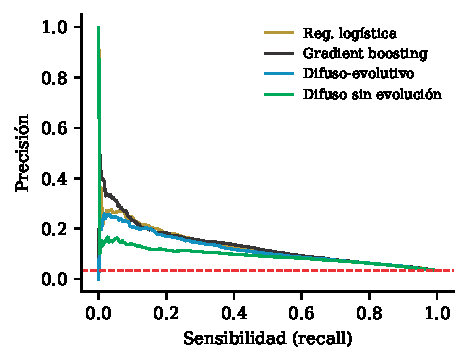
\includegraphics[width=0.9\columnwidth]{../../resultados/figuras/curvas_pr.pdf}
\caption{Curvas de precisión-sensibilidad en la prueba de 2026 (semilla de referencia). La línea roja es la prevalencia.}
\label{fig:pr}
\end{figure}

\subsection{Robustez y análisis de errores}

\textbf{Degradación dentro de 2026} (Fig.~\ref{fig:mes}). Todos los modelos se degradan a lo largo del año. El difuso-evolutivo baja de \cifMesIni{} en enero a \cifMesFin{} en julio, y el \emph{gradient boosting} de \cifMesGBIni{} a \cifMesGBFin{}. La deriva crece a medida que la prueba se aleja del entrenamiento.

\textbf{Subgrupo \texttt{Assisted-by}} (\cifAssistedN{} commits, prevalencia \cifAssistedPrev{}). Es descriptivo, porque la etiqueta es una cota inferior. Todos los modelos rinden peor que en el resto:
\begin{itemize}
\item difuso-evolutivo: \cifAssistedFE{} frente a \cifSinAssistedFE{};
\item \emph{gradient boosting}: \cifAssistedGB{} frente a \cifSinAssistedGB{};
\item regresión logística: \cifAssistedLR{} frente a \cifSinAssistedLR{}.
\end{itemize}
Las señales de tamaño y difusión que funcionan en general predicen menos en los commits declarados como asistidos.

\textbf{Errores por tipo de commit.} Los errores del difuso se concentran en dos grupos:
\begin{itemize}
\item \textbf{Commits pequeños.} En los tres quintiles inferiores de líneas añadidas la sensibilidad es 0: las reglas nunca los marcan. En el quintil superior (prevalencia \cifErrQcincoPrev{}) detecta el \cifErrQcincoSens{} de los riesgosos.
\item \textbf{Correcciones.} En los commits que traen su propio \texttt{Fixes:}, el AUC-PR es \cifErrFixAp{} frente a \cifErrNoFixAp{}, y la sensibilidad \cifErrFixSens{} frente a \cifErrNoFixSens{}. Una corrección que introduce otro error suele ser pequeña.
\end{itemize}

\begin{figure}[!t]
\centering
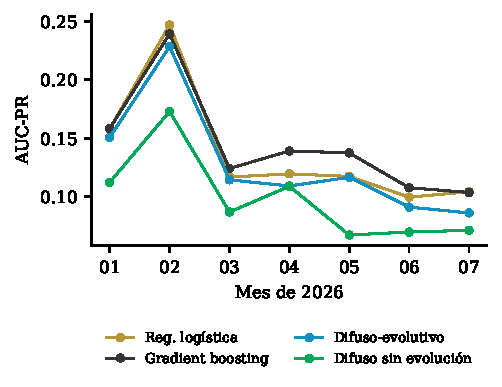
\includegraphics[width=0.95\columnwidth]{../../resultados/figuras/auc_pr_por_mes.pdf}
\caption{AUC-PR por mes de 2026 (semilla de referencia).}
\label{fig:mes}
\end{figure}

\subsection{Interpretabilidad: las reglas aprendidas}

El modelo de la semilla de referencia tiene \cifNReglasRef{} reglas (Tabla~\ref{tab:reglas}) y \cifParamFE{} parámetros en promedio entre semillas, frente a \cifParamGBprueba{} del \emph{gradient boosting}. Cada término se resume con su corte $\alpha=0{,}5$ en unidades originales.

Las reglas se leen solas:
\begin{itemize}
\item un cambio que agrega muchas líneas es sospechoso (R1), más aún si toca varios archivos (R2);
\item también lo es el que toca más de un subsistema (R4, R5);
\item con menos peso, el código nuevo puro: un solo subsistema y nada borrado (R3).
\end{itemize}
Coinciden con las familias de tamaño y difusión de la literatura JIT \cite{Kamei2013}. En esta semilla, la revisión (\texttt{Reviewed-by}) y la experiencia del autor no sobrevivieron a la evolución.

\begin{table}[!t]
\caption{Base de reglas del difuso-evolutivo (semilla de referencia). Entre paréntesis, el corte $\alpha=0{,}5$ de cada término}
\label{tab:reglas}
\centering\footnotesize
\begin{tabularx}{\columnwidth}{@{}c c Y@{}}
\toprule
\cabecera & \textbf{Peso} & \textbf{SI \ldots\ ENTONCES riesgoso}\\
\midrule
\filas{../comun/tabla_reglas.tex}
\bottomrule
\end{tabularx}
\end{table}

\textbf{Aporte de la evolución.} En la prueba, la evolución sube el AUC-PR un \cifAporteEvolPrueba{} frente a la variante sin evolución (\cifTestFE{} frente a \cifTestVar{}), y reduce el modelo de \cifReglasVariante{} reglas a 3--6.
